\documentclass[11pt,a4paper,twocolumn]{article}

% === Core Packages ===
\usepackage[margin=2cm]{geometry}
\usepackage[utf8]{inputenc}
\usepackage[T1]{fontenc}
\usepackage{times}
\usepackage{amsmath,amssymb}
\usepackage{graphicx}
\usepackage{booktabs}
\usepackage{float}
\usepackage{enumitem}
\usepackage{tikz}
\usepackage{pgfplots}
\pgfplotsset{compat=1.18}
\usetikzlibrary{arrows.meta,shapes.geometric,positioning,calc,decorations.markings,fit,backgrounds}

% === Citation (IEEE style) ===
\usepackage[numbers,sort&compress]{natbib}
\bibliographystyle{IEEEtranN}

% === Hyperref ===
\usepackage[hidelinks]{hyperref}
\usepackage{xurl}

% === Settings ===
\setlength{\parindent}{1em}
\setlength{\parskip}{0.3em}

% === Title ===
\title{\textbf{Desentralisert omdømmenettverk:\\Et rammeverk for naturlig samfunnsorganisering}}
\author{Pavel Kudrna\\Prague, Czechia\\Utkast v1 --- mars 2026}
\date{}

\begin{document}
\maketitle

% ============================================================
% ABSTRACT
% ============================================================
\begin{abstract}
Rettferdighetssansen---overbevisningen om at urett blir rettet opp og at fortjeneste blir belønnet---er samfunnets sterkeste samlende kraft. Når sentraliserte styringsinstitusjoner ikke kan levere denne følelsen fordi kostnaden ved å håndheve en rettighet overstiger verdien av rettigheten selv, forvitrer den sosiale samholdet. Nåværende institusjonelle strukturer klarer ikke å løse en betydelig klasse av tvister på systematisk samme måte som sentral planlegging svikter i å fordele ressurser: gjennom informasjonsasymmetri, manglende tilbakekoblingssløyfer og frakobling av beslutningstakere fra konsekvensene av sine beslutninger. Denne artikkelen presenterer et omdømmebasert sosialt nettverk (Reputation Social Network, RSN): et desentralisert, ubestikkelig og sensurbestandig kommunikasjonslag bygget på desentraliserte identifikatorer (DID-er) som gjør det mulig for pseudonyme deltakere å publisere, verifisere og konsumere omdømmeinformasjon om atferd i den virkelige verden. Kjernemekanismen hviler på tre designprinsipper: (1)~en asymmetrisk kostnadsstruktur der lesing av omdømmedata er billig, men skriving krever verifiserbar innsats; (2)~en ikke-deterministisk protokoll for valg av verifikatorer basert på konsistent hashing som priser radikale påstander gjennom eskalerende iterasjonskostnader; og (3)~en markedsdrevet modell for omdømmeautoriteter der private verifikatorer setter sitt akkumulerte omdømme på spill for nøyaktigheten av påstandene de bekrefter. Den resulterende arkitekturen frembringer et emergent meritokrati uten sentral koordinering og muliggjør en gradvis, reverserbar migreringsvei fra eksisterende statsadministrerte systemer.
\end{abstract}

% ============================================================
% 1. INTRODUCTION
% ============================================================
\section{Innledning}

\subsection{Problemet med sentralisert tillit}

Moderne styring hviler på en grunnleggende antakelse: at sentraliserte institusjoner kan formidle tillit mellom fremmede i stor skala. Domstoler avgjør tvister. Registre sertifiserer eierskap. Tilsynsorganer håndhever standarder. Disse institusjonene ble utformet i en tid da informasjon var knapp, kommunikasjon var langsom, og delegering av myndighet til et sentralt organ var den eneste gjennomførbare koordineringsmekanismen. Sentralisert styring svikter imidlertid av de samme strukturelle grunnene som sentral planlegging: informasjonsasymmetri, manglende tilbakekoblingssløyfer og frakobling av beslutningstakere fra konsekvensene av sine beslutninger.

Antakelsen svikter for eksempel når kostnaden ved institusjonell formidling overstiger verdien av tvisten. Tenk på en leietaker som oppdager at den leide leiligheten mangler et lovpålagt elektrisk sikkerhetssertifikat---en tilstand som utgjør en umiddelbar livsfare. Leietakerens juridiske rett til å trekke seg fra kontrakten er utvetydig. Likevel overstiger kostnaden ved å håndheve denne rettigheten gjennom rettssystemet den pengemessige verdien av depositumet og erstatningen som skyldes, selv om man inkluderer potensiell lovbestemt kompensasjon~\cite{czcourtfees}. Den rasjonelle responsen er å bære tapet og trekke seg ut.

Dette er ikke et patologisk grensetilfelle. Det er standarderfaringen for en betydelig klasse av tvister der skaden er reell, men de pengemessige innsatsene faller under terskelen der institusjonell håndheving blir økonomisk rasjonell. Resultatet er et system som strukturelt favoriserer aktører med onde hensikter: de som skader andre i volumer under denne terskelen kan handle ustraffet, fordi kostnaden ved å søke rettferdighet faller på den skadelidte parten.

Eksempelet ovenfor er hentet fra forfatterens juridiske miljø---det tsjekkiske sivilrettssystemet. I andre rettstradisjoner---presedensbasert sedvanerett (common law), sedvanerett, blandede systemer---svikter rettferdigheten på ulike måter og i ulik grad, avhengig av de kulturelle og prosessuelle særtrekkene ved jurisdiksjonen. Lesere vil sannsynligvis kjenne igjen tilsvarende eksempler fra sin egen kontekst. Det som er strukturelt universelt, er mønsteret: tvister hvis verdi faller under terskelen for økonomisk rasjonell håndheving ender med at tapet bæres av den skadelidte parten. RSN lover ikke perfekt rettferdighet---den reduserer bare den strukturelle fordelen som aktører med onde hensikter nyter godt av når institusjonell håndheving er ulønnsom.

\subsection{Hvorfor eksisterende løsninger kommer til kort}

\textbf{Rammeverk for desentralisert identitet (DID)}~\cite{did2022} tilbyr kryptografiske mekanismer for selvsuveren identitetsforvaltning, men fokuserer primært på identitetsverifisering uten å adressere det bredere spørsmålet om atferdsmessig omdømme.

\textbf{Soulbound-token (SBT-er)}~\cite{weyl2022} fanger innsikten om at omdømme er ikke-overførbart, men er avhengige av blokkjede-infrastruktur med skaleringsbegrensninger og adresserer ikke de økonomiske insentivene som styrer informasjonsinngang. Beslektede konsepter som fortjenestetoken (f.eks. Liberland) deler en lignende filosofi, men forblir bundet til spesifikke jurisdiksjonelle rammeverk.

\textbf{Desentraliserte autonome organisasjoner (DAO-er)}~\cite{buterin2014} implementerer styring gjennom smartkontrakter, men reproduserer plutokratiske dynamikker der innflytelse er proporsjonal med kapital. Kvadratisk stemmegivning~\cite{buterin2019} demper dette delvis, men begrenser praktisk adopsjon. DAO-er står også overfor det grunnleggende \emph{orakelproblemet}: smartkontrakter kan ikke pålitelig verifisere tilstander i den virkelige verden uten en pålitelig ekstern kilde, og dette problemet har ingen generell løsning innenfor blokkjedearkitektur.

Ingen eksisterende system kombinerer desentralisering, sensurbestandighet, pseudonymitet, verifiserbar inngangskostnad og emergent konsensus.

\subsection{Bidrag}

Denne artikkelen gir følgende bidrag:
\begin{enumerate}[nosep]
\item Definisjon av \textbf{omdømmebasert sosialt nettverk (RSN)}, en desentralisert protokoll som utvider DID-rammeverket til å støtte bilateral omdømmeutveksling.
\item En \textbf{ikke-deterministisk protokoll for valg av verifikatorer} basert på konsistent hashing~\cite{karger1997}.
\item \textbf{Prinsippet om kostbar radikalisme}, som priser påstander etter deres avstand fra nettverkskonsensus gjennom tre sammensatte kostnadskanaler.
\item En \textbf{modell for anerkjente autoriteter} med asymmetriske insentiver der falsk bekreftelse koster katastrofalt mye mer enn legitime gebyrer.
\item En \textbf{gradvis migreringsvei} gjennom parallell finanspolitisk infrastruktur.
\end{enumerate}

% ============================================================
% 2. DESIGN PRINCIPLES
% ============================================================
\section{Designprinsipper}

RSN-arkitekturen er begrenset av fem ikke-forhandlingsbare designprinsipper.

\textbf{Kontinuitet og evolusjon.} Systemet eksisterer side om side med eksisterende institusjoner i en overgangsperiode av ubestemt lengde. Overgangen må være reverserbar på hvert trinn.

\textbf{Frivillighet og ansvar.} Deltakelse er frivillig, men frivilligheten er koblet til ansvar: en deltaker som tar kontroll over en institusjonell funksjon, påtar seg samtidig de tilhørende forpliktelsene.

\textbf{Mangfold og kulturell nøytralitet.} Konsensus oppstår fra bilaterale interaksjoner, ikke fra forhåndsdefinerte regler pålagt av systemdesignere.

\textbf{Robusthet og sensurbestandighet.} Kostnaden ved å sensurere nettverket må overstige kostnaden ved å tolerere det. Kun fullstendig totalitarisme---til ruinerende politiske og økonomiske kostnader---kan undertrykke systemet.

\textbf{Konsensus og håndheving.} Systemet innlemmer menneskelige tilbøyeligheter til smålighet, ondskap og gjengjeldende tilfredsstillelse som bærende egenskaper. Uredelighet er ikke forbudt; den prises.

% ============================================================
% 3. SYSTEM OVERVIEW
% ============================================================
\section{Systemoversikt}

\subsection{Omdømmebasert sosialt nettverk}

RSN er et desentralisert kommunikasjonslag av typen node-til-node (peer-to-peer) der deltakere utveksler verifiserbar informasjon om atferd i den virkelige verden. Dets definerende egenskaper er: desentralisert og usensurerbar infrastruktur; pseudonym deltakelse gjennom DID-er; asymmetrisk kostnadsstruktur (lesing er billig, skriving er kostbar); kryptografisk verifiserbarhet; og \textbf{standardstøtte}---maskinlesbare formater for informasjon som spres gjennom nettverket, for tjenester tilbudt av autoriteter (sammensetning av påstander, bekreftelse, vitnetjeneste), og for policyformatet inkludert regler for evaluering av motpartens omdømme og vurdering av risikoen for policy-avvik (mellom erklært og faktisk atferd).

\subsection{Arkitektoniske komponenter}

RSN består av fire primære komponenter (Fig.~\ref{fig:architecture}):
\begin{enumerate}[nosep]
\item \textbf{DID-lag.} Deltakeridentiteter med erklærte regler, omdømmemetadata og nettverksruting.
\item \textbf{Påstandsprotokoll.} Strukturert format for å publisere utsagn om hendelser i den virkelige verden.
\item \textbf{Verifikasjonsnettverk.} Desentralisert protokoll for å tildele verifikatorer ved hjelp av konsistent hashing.
\item \textbf{Aggregeringslag for omdømme.} Tjenester som produserer menneskelesbare omdømmesammendrag.
\end{enumerate}

\begin{figure}[ht]
\centering
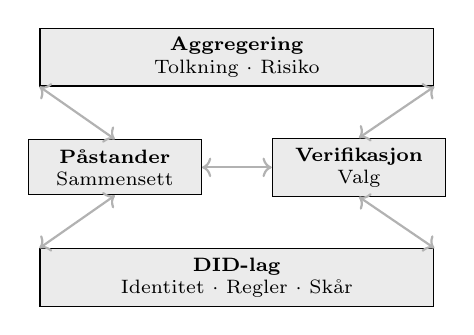
\begin{tikzpicture}[
    layer/.style={draw, minimum height=0.7cm, align=center, font=\scriptsize, fill=black!8},
    arr/.style={<->, thick, gray!60}
]
\node[layer, minimum width=5cm] (agg) at (0,2.8) {\textbf{Aggregering}\\Tolkning $\cdot$ Risiko};
\node[layer, minimum width=2.2cm] (claim) at (-1.55,1.4) {\textbf{Påstander}\\Sammensett};
\node[layer, minimum width=2.2cm] (verif) at (1.55,1.4) {\textbf{Verifikasjon}\\Valg};
\node[layer, minimum width=5cm] (did) at (0,0) {\textbf{DID-lag}\\Identitet $\cdot$ Regler $\cdot$ Skår};

\draw[arr] (agg.south west) -- (claim.north);
\draw[arr] (agg.south east) -- (verif.north);
\draw[arr] (claim.east) -- (verif.west);
\draw[arr] (claim.south) -- (did.north west);
\draw[arr] (verif.south) -- (did.north east);
\end{tikzpicture}
\caption{RSN firelags arkitektur.}
\label{fig:architecture}
\end{figure}

\subsection{Deltakerroller}

En verifikasjonstransaksjon involverer opptil seks distinkte DID-roller (Fig.~\ref{fig:roles}): \textbf{Utsteder} ($DID_I$, oppretter og sender inn påstanden), \textbf{Subjekt} ($DID_S$, DID-en påstanden handler om---kan sammenfalle med Utsteder), \textbf{Autoritet} ($DID_A$, bekrefter påstanden mot et gebyr; kan også tilby vitnetjenester---\emph{valgfritt}), \textbf{Vitne} ($DID_{W_{1..n}}$, inkognito overvåker av verifikatorens ærlighet via utfordringskoder---\emph{valgfritt}), \textbf{Verifikator} ($DID_V$, algoritmisk valgt til å publisere påstanden), og \textbf{RSN} (nettverket der verifiserte påstander publiseres). Enhver rolle kan delegeres til en annen DID (avsnitt~7.4). En Autoritet bunter vanligvis sammen bekreftelse med vitnetjenester, men de to funksjonene er logisk uavhengige.

\begin{figure}[ht]
\centering
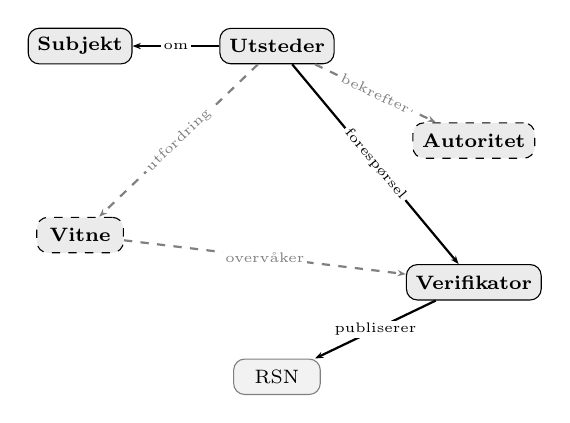
\begin{tikzpicture}[
    role/.style={draw, rounded corners, minimum width=1.1cm, minimum height=0.45cm, align=center, font=\scriptsize, fill=black!8},
    opt/.style={draw, rounded corners, minimum width=1.1cm, minimum height=0.45cm, align=center, font=\scriptsize, fill=black!8, dashed},
    arr/.style={-{Stealth[length=3pt]}, thick},
    oarr/.style={-{Stealth[length=3pt]}, thick, dashed, gray},
    lbl/.style={font=\tiny, fill=white, inner sep=1pt}
]
\node[role] (I) at (0,2.4) {\textbf{Utsteder}};
\node[role] (S) at (-2.5,2.4) {\textbf{Subjekt}};
\node[opt] (A) at (2.5,1.2) {\textbf{Autoritet}};
\node[opt] (W) at (-2.5,0) {\textbf{Vitne}};
\node[role] (V) at (2.5,-0.6) {\textbf{Verifikator}};
\node[role, fill=black!5, draw=gray] (N) at (0,-1.8) {RSN};

\draw[arr] (I) -- node[lbl] {om} (S);
\draw[oarr] (I) -- node[lbl,sloped] {bekrefter} (A);
\draw[oarr] (I) -- node[lbl,sloped] {utfordring} (W);
\draw[arr] (I) -- node[lbl,sloped] {forespørsel} (V);
\draw[oarr] (W) -- node[lbl] {overvåker} (V);
\draw[arr] (V) -- node[lbl] {publiserer} (N);
\end{tikzpicture}
\caption{DID-roller i en verifikasjonstransaksjon. Stiplet = valgfritt (Autoritet, Vitne).}
\label{fig:roles}
\end{figure}

\subsection{Ubestikkelighet: Fire krefter}

RSN-ets ubestikkelighet oppstår ikke fra en enkelt mekanisme, men fra fire samtidige krefter. Ingen er tilstrekkelig i seg selv; bare deres kombinasjon gjør et korrupsjonsforsøk økonomisk irrasjonelt.

\textbf{Uforutsigbart mål.} Verifikatoren for hver påstand velges ikke-deterministisk gjennom konsistent hashing (avsnitt~5.3). En angriper kan ikke på forhånd sikte seg inn på en spesifikk verifikator for bestikkelse, fordi verifikatorens identitet er en funksjon av påstandens innhold og tidligere iterasjoner, ikke av utstederens valg.

\textbf{Omdømmemessig innflytelse---langsomt opp, raskt ned.} Omdømme kan bare bygges gradvis, gjennom vedvarende konsistent atferd. Det kan imidlertid gå tapt katastrofalt i en enkelt svindelaktig bekreftelse (avsnitt~6.2). Denne asymmetrien betyr at år med akkumulert omdømme kan ødelegges av én uærlig bekreftelse; den optimale strategien forblir å avvise mistenkelige påstander.

\textbf{Offentlig løfte.} Hver DID-innehaver erklærer offentlig sin policy---et maskinlesbart sett med regler de forplikter seg til å følge. Avvik mellom erklæringen og faktisk atferd er oppdagbart og prises som en omdømmeforseelse mer alvorlig enn den underliggende overtredelsen (avsnitt~7.3). Hykleri er derfor mer kostbart enn direkte uærlighet.

\textbf{Nettverksmessig asymmetri i angrepskostnad.} Kostnaden ved å sensurere eller destabilisere nettverket vokser ikke-lineært med nettverkets størrelse og tetthet, mens kostnaden ved å tolerere det forblir konstant. For at sensur skal lønne seg, måtte en sentralisert aktør anvende den på tvers av hele nettverket---noe som krever tiltak uproporsjonale med enhver tenkelig fordel (avsnitt~10).

% ============================================================
% 4. DECENTRALIZED IDENTITY MODEL
% ============================================================
\section{Modell for desentralisert identitet}

\subsection{DID med spesielle egenskaper}

RSN utvider W3C DID Core-spesifikasjonen~\cite{did2022} med: \textbf{Erklærte regler} (maskinlesbare atferdsforpliktelser), \textbf{Omdømmemetadata} (aggregert atferdsskår) og \textbf{Nettverksruting} (foranderlig onion-gateway atskilt fra den stabile ringposisjonen).

\subsection{Påstandens livssyklus}

En påstand går gjennom seks stadier (Fig.~\ref{fig:lifecycle}): sammensetning, valgfri autoritetsbekreftelse, valg av verifikator via konsistent hashing, verifikasjonsbeslutning (godta eller avvis med iterasjon), publisering og omdømmeoppdatering for alle parter.

\begin{figure}[ht]
\centering
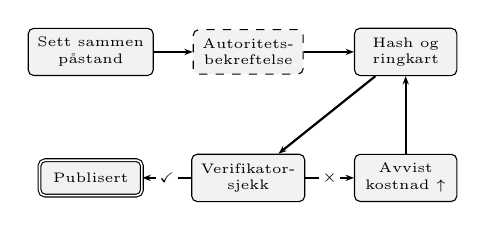
\begin{tikzpicture}[
    stp/.style={draw, rounded corners=2pt, minimum width=1.3cm, minimum height=0.45cm, align=center, font=\tiny, fill=black!5},
    arr/.style={-{Stealth[length=3pt]}, thick},
    lbl/.style={font=\tiny, fill=white, inner sep=1pt}
]
\node[stp] (comp) at (0,0) {Sett sammen\\påstand};
\node[stp, dashed] (auth) at (2.0,0) {Autoritets-\\bekreftelse};
\node[stp] (hash) at (4.0,0) {Hash og\\ringkart};
\node[stp] (ver) at (2.0,-1.6) {Verifikator-\\sjekk};
\node[stp, double] (pub) at (0,-1.6) {Publisert};
\node[stp] (rej) at (4.0,-1.6) {Avvist\\kostnad $\uparrow$};

\draw[arr] (comp) -- (auth);
\draw[arr] (auth) -- (hash);
\draw[arr] (hash) -- (ver);
\draw[arr] (ver) -- node[lbl] {\checkmark} (pub);
\draw[arr] (ver) -- node[lbl] {$\times$} (rej);
\draw[arr] (rej) -- ++(0,0.8) -| (hash);
\end{tikzpicture}
\caption{Påstandens livssyklus med iterasjonssløyfe.}
\label{fig:lifecycle}
\end{figure}

\subsection{Forhold til W3C DID Core}

RSN-ets identitetsmodell er et ekte supersett av W3C DID Core-spesifikasjonen~\cite{did2022}. Alle RSN DID-er er gyldige W3C DID-er. De RSN-spesifikke utvidelsene er kodet som egenskaper i DID-dokumentet, definert i en dedikert DID-metodespesifikasjon, kompatibel med eksisterende infrastruktur som ION~\cite{buchner2021} og Ceramic~\cite{ceramic2023}.

% ============================================================
% 5. VERIFICATION AND PROPAGATION
% ============================================================
\section{Verifisering og spredning av informasjon}

\subsection{Kostnaden ved informasjonsinngang}

RSN-ets økonomiske kjerneprinsipp er asymmetrien mellom lesing og skriving. Lesing av omdømmedata nærmer seg null marginalkostnad for deltakere som er en del av DID-nettverket og har tilgang som står i forhold til sitt omdømme---nykommere må gradvis fortjene bredere tilgang (se anti-snylting). Skriving---forstått som den varige materialiseringen av omdømme inn i nettverket, ikke som en engangs teknisk handling---krever verifiserbar kumulativ investering på tvers av tre dimensjoner: \textbf{tid} (leveår brukt på konsistent atferd, oppfylte forpliktelser og kultiverte relasjoner), \textbf{energi} (innsats lagt i ærlig handel, omsorg for partnerskap og langsiktig troverdighet), og \textbf{penger} (investering i eget navn---faglig utvikling, kvaliteten på ens arbeid, gjenoppretting av forvoldte skader). Omdømme kan ikke kjøpes umiddelbart---det er resultatet av livslang akkumulering som systemet bare gjør synlig og overførbart på tvers av kontekster. De teknisk engangskostnadene ved protokollen (kryptografiske signaturer, verifikatorgebyrer) er ubetydelige sammenlignet med denne underliggende investeringen.

\subsection{Sosial graf og kontaktdybde}

RSN er fundamentalt et sosialt nettverk: hver DID legger til kontakter (andre DID-er) som tillater forbindelsen. Disse kontaktene har sine egne kontakter, og så videre. Det algoritmiske søket etter verifikatorer opererer innenfor en konfigurerbar dybde $h$ av tilknyttede kontakter (f.eks. $h=3$: ens direkte kontakter, deres kontakter, og kontakters kontakter). Denne arkitekturen krever ikke en enkelt global blokkjede---den favoriserer naturlig fremveksten av fellesskap/klynger med overlapp inn i andre fellesskap. Hver DID-deltaker må ha en publisert \textbf{policy}---et maskinlesbart sett med regler som styrer hvordan innkommende forespørsler evalueres. Policybrudd registreres i nettverket som negative artefakter.

\subsection{Algoritmisk valg av verifikator}

Verifikasjonsprotokollen benytter konsistent hashing~\cite{karger1997} (Fig.~\ref{fig:verifier}). Verifisering er en betalt tjeneste: verifikatorer opererer mot et gebyr, noe som skaper et marked der konkurranse driver prising, hastighet og pålitelighet.

\textbf{Trinn 1.} Påstandsdokumentet sammenkjedes med hashresultatet fra forrige iterasjon (eller $\varnothing$ ved første iterasjon) og hashes:
\begin{equation}
\text{pos} = f_h(\text{claim} \| \text{prev\_hash})
\label{eq:hash}
\end{equation}

Algoritmen må inkludere den \emph{fullstendige stien} av alle tidligere forespørsler og svar---ikke bare en hash av forrige iterasjon. Hver verifikators fullstendige svar (aksept, avvisning, oppgitt pris, begrunnelse) legges til det voksende dokumentet, verifiserbart gjennom kryptografiske signaturer i hvert trinn.

\textbf{Trinn 2.} Hashen kartlegges til $N$ posisjoner på den konsistente hashringen, jevnt fordelt (f.eks. for $N=4$: $+0^{\circ}, +90^{\circ}, +180^{\circ}, +270^{\circ}$). Fra hver posisjon velger et søk med klokken den nærmeste DID-en som verifikatorkandidat (Fig.~\ref{fig:multipoint}). $N$ er en variabel parameter som kan avhenge av prosentandelen av for øyeblikket aktive DID-er, tid på døgnet eller historisk nettverksrespons.

\textbf{Trinn 3.} Verifikatoren godtar (publiserer, setter omdømme på spill) eller avviser (returnerer til trinn~1 med avvisningshashen). Når en node ikke svarer til tross for erklært tilkoblingsstatus, må neste forespørsel inkludere alle svar fra alle $N$ tidligere verifikatorkandidater.

\textbf{Anti-snylting.} Mål-DID-er kan sette gebyrer eller tilgangsbegrensninger for spørringer fra nye DID-er med lite omdømme. Denne graderte mekanismen (ikke binær) tvinger nykommere til å bygge omdømme gjennom genuin aktivitet før de fritt kan konsumere andres data.

\begin{figure}[ht]
\centering
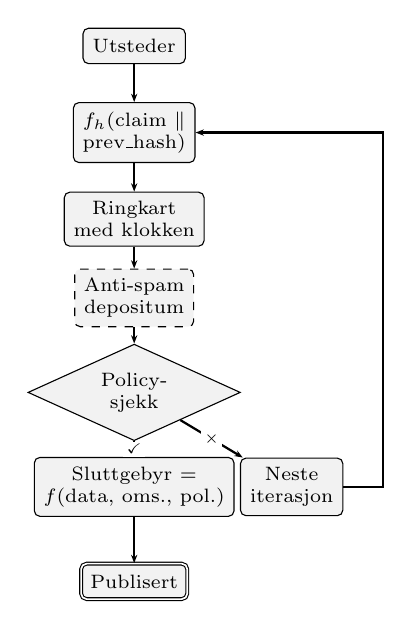
\begin{tikzpicture}[
    box/.style={draw, rounded corners=2pt, minimum width=1.3cm, minimum height=0.45cm, align=center, font=\scriptsize, fill=black!5},
    dec/.style={draw, diamond, aspect=2.2, minimum width=0.9cm, align=center, font=\scriptsize, fill=black!5},
    arr/.style={-{Stealth[length=3pt]}, thick},
    lbl/.style={font=\tiny, fill=white, inner sep=1pt}
]
\node[box] (iss) at (0,0) {Utsteder};
\node[box] (hash) at (0,-1.1) {$f_h$(claim $\|$\\prev\_hash)};
\node[box] (ring) at (0,-2.2) {Ringkart\\med klokken};
\node[box, dashed] (spam) at (0,-3.2) {Anti-spam\\depositum};
\node[dec] (check) at (0,-4.4) {Policy-\\sjekk};
\node[box] (rej) at (2,-5.6) {Neste\\iterasjon};
\node[box] (fee) at (0,-5.6) {Sluttgebyr =\\$f$(data, oms., pol.)};
\node[box, double] (pub) at (0,-6.8) {Publisert};

\draw[arr] (iss) -- (hash);
\draw[arr] (hash) -- (ring);
\draw[arr] (ring) -- (spam);
\draw[arr] (spam) -- (check);
\draw[arr] (check) -- node[lbl] {$\times$} (rej);
\draw[arr] (check) -- node[lbl] {\checkmark} (fee);
\draw[arr] (fee) -- (pub);
\draw[arr] (rej.east) -- ++(0.5,0) |- (hash.east);
\end{tikzpicture}
\caption{Protokoll for valg av verifikator. Anti-spam-depositum er valgfritt og kan være refunderbart. Sluttgebyret betales kun ved aksept.}
\label{fig:verifier}
\end{figure}

Hver avvisning legger verifikatorens fullstendige svar (inkludert begrunnelser og betingelser) til påstandsdokumentet, og utvider dets innhold. Fra det utvidede dokumentet beregnes en ny hash ikke-deterministisk, som kartlegges til en annen ringposisjon og velger en annen verifikator. Dokumentasjon av den fullstendige stien er obligatorisk---utstederen kan ikke forutsi eller påvirke neste verifikator. Hvis en verifikator ignorerer en forespørsel til tross for en kompatibel erklært policy, registrerer vitner (hvis til stede) dette, og utstederen kan vedlegge vitnebevis ved endelig publisering.

\begin{figure}[ht]
\centering
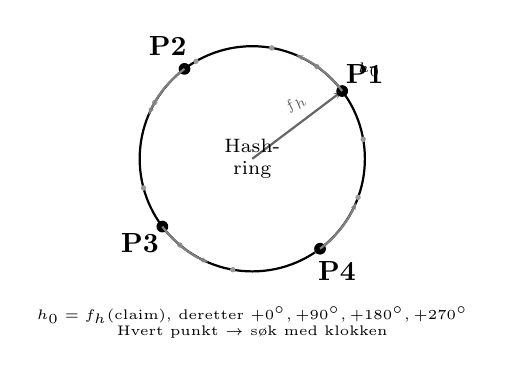
\begin{tikzpicture}[scale=0.65]
% Ring
\draw[thick] (0,0) circle (2.2cm);
% DID nodes on ring
\foreach \a in {10,55,80,120,150,195,230,260,305,340} {
  \fill[black!40] (\a:2.2) circle (1.5pt);
}
% Hash offset arrow pointing to initial position
\draw[-{Stealth[length=3pt]}, thick, black!60] (0,0) -- node[font=\tiny,above,sloped,pos=0.6] {$f_h$} (37:2.2);
\fill[black] (37:2.2) circle (2pt);
\node[font=\tiny,anchor=south west] at (37:2.35) {$h_0$};
% N=4 points offset from h0 by +0, +90, +180, +270
\foreach \offset/\l in {0/P1,90/P2,180/P3,270/P4} {
  \pgfmathsetmacro{\ang}{37+\offset}
  \node[fill=black, circle, inner sep=1.5pt] (p\offset) at (\ang:2.2) {};
  \node[font=\tiny,font=\bfseries] at (\ang:2.75) {\l};
  % clockwise search arc
  \draw[-{Stealth[length=2.5pt]}, thick, gray] (\ang:2.2) arc (\ang:\ang+30:2.2);
}
\node[font=\scriptsize, align=center] at (0,0) {Hash-\\ring};
\node[font=\tiny, align=center] at (0,-3.2) {$h_0 = f_h(\text{claim})$, deretter $+0^{\circ},+90^{\circ},+180^{\circ},+270^{\circ}$\\Hvert punkt $\rightarrow$ søk med klokken};
\end{tikzpicture}
\caption{Flerpunktsvalg ($N{=}4$). Hash $h_0$ setter forskyvningen; 4 punkter jevnt fordelt fra $h_0$.}
\label{fig:multipoint}
\end{figure}

\subsection{Vitneprotokoll}

\textbf{Vitne}-rollen gir inkognito ansvarliggjøring for verifikatorens ærlighet gjennom en kryptografisk protokoll med utfordringskoder:

\textbf{Trinn V1.} Forespørreren signerer verifikasjonsforespørselen og sender den til $N_w$ vitner---kontakter fra forespørrerens sosiale nettverk, eller spesialiserte leverandører av vitnetjenester som opererer mot et gebyr.

\textbf{Trinn V2.} Hvert vitne $w_i$ signerer hele den signerte forespørselen, beholder den opprinnelige signaturen $\sigma_i$, og beregner en utfordringskode $c_i = h(\sigma_i)$. Utfordringskoden legges til forespørselen.

\textbf{Trinn V3.} Forespørselen, som nå bærer $N_w$ utfordringskoder, sendes til verifikatoren. Verifikatoren observerer kodene, men \emph{kan ikke fastslå} hvem vitnene er, eller om kodene tilsvarer reelle signaturer.

\textbf{Trinn V4 (ærlig verifikator).} Hvis verifikatoren svarer i tråd med sin erklærte policy, forblir utfordringskodene ugjennomsiktige. Vitner avsløres aldri. Ingen tilleggsdata publiseres.

\textbf{Trinn V5 (policybrudd).} Hvis verifikatoren bryter sin policy (ignorerer forespørselen, svarer inkonsekvent), holder forespørreren vitnenes opprinnelige signaturer $\sigma_i$. Disse kan publiseres som følgedata: hvem som helst kan verifisere $c_i = h(\sigma_i)$, og bevise at vitnet var til stede. Forespørreren kan publisere uavhengig---verifikatoren har allerede signert utfordringskodene i sitt svar.

\textbf{Bløff-egenskapen.} Forespørreren kan erstatte noen eller alle utfordringskoder med tilfeldige verdier. Verifikatoren kan ikke skille genuine koder (støttet av autoriteter med høyt omdømme) fra støy. Denne \emph{usikkerheten} er håndhevingsmekanismen: hver forespørsel bærer risikoen for at en respektert autoritet ser på inkognito. Kostnaden ved å opprettholde dette presset er nær null (generering av tilfeldige tall), mens den potensielle kostnaden ved uærlighet for verifikatoren er katastrofal. Ærlig atferd insentiveres selv i fravær av faktiske vitner.

\textbf{Autoritet som vitne.} En Autoritet som bekrefter en påstand, kan bunte sammen vitnetjenester: ``Jeg bekrefter din påstand og fungerer som inkognito vitne under verifiseringen.'' Dette er en naturlig forretningsmodell---Autoriteten har allerede konteksten. De to rollene er imidlertid logisk uavhengige.

\subsection{Prinsippet om kostbar radikalisme}

Tre kostnadskanaler sammensettes samtidig (Fig.~\ref{fig:radicalism}):

\textbf{Kanal 1: Iterasjonskostnad.} Hver avvisning tvinger frem en ny iterasjon som forbruker tid og ressurser. Lineær vekst.

\textbf{Kanal 2: Dokumentoppsvulming.} Hver iterasjon legger verifikatorens fullstendige svar til påstandsdokumentet. Veksten er lineær, men med en basisforskyvning: den innledende nyttelasten (påstandsinnhold, autoritetsbekreftelse, kryptografiske signaturer) har allerede en ikke-triviell størrelse $B_0$. Total størrelse etter $k$ iterasjoner: $S(k) = B_0 + k \cdot \Delta$, der $\Delta$ er gjennomsnittlig svarstørrelse.

\textbf{Kanal 3: Verifikatorens risikopremie.} Risiko er subjektiv. Verifikatoren vurderer om den forespørrende DID-ens erklærte policyer er i konflikt med verifikatorens egne kommersielle, sosiale eller politiske interesser. Premien kan eskalere eksponentielt med opplevd avstand fra verifikatorens ``ideal'': $P(d) = \alpha \cdot e^{\beta d}$, der $d$ er verifikatorens subjektive avstandsmetrikk. Utover en personlig no-go-grense kan verifikatoren nekte fullstendig.

\begin{figure}[ht]
\centering
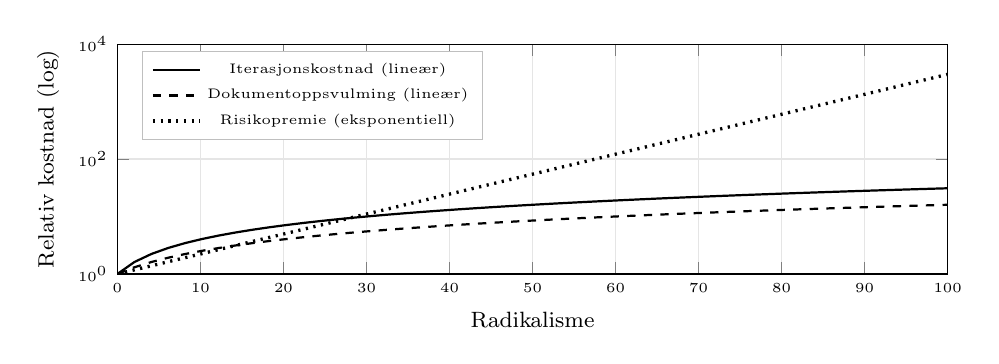
\begin{tikzpicture}
\begin{axis}[
    width=\columnwidth,
    height=4.5cm,
    xlabel={\footnotesize Radikalisme},
    ylabel={\footnotesize Relativ kostnad (log)},
    ymode=log,
    xmin=0, xmax=100,
    ymin=1, ymax=10000,
    grid=major,
    grid style={gray!20},
    legend style={at={(0.03,0.97)},anchor=north west,font=\tiny,draw=gray!50},
    tick label style={font=\tiny},
    label style={font=\footnotesize},
]
\addplot[black, thick, domain=0:100, samples=50] {1 + 0.3*x};
\addlegendentry{Iterasjonskostnad (lineær)}
\addplot[black, thick, dashed, domain=0:100, samples=50] {1 + 0.15*x};
\addlegendentry{Dokumentoppsvulming (lineær)}
\addplot[black, thick, dotted, line width=1.2pt, domain=0:100, samples=100] {exp(0.08*x)};
\addlegendentry{Risikopremie (eksponentiell)}
\end{axis}
\end{tikzpicture}
\caption{Kostnadseskalering på tvers av tre kanaler. Risikopremien dominerer ved høy radikalisme.}
\label{fig:radicalism}
\end{figure}

Kritisk nok er dette ikke sensur. Ingen påstand er forbudt. Systemet priser risiko (Tabell~\ref{tab:costs}).

\begin{table}[ht]
\centering
\caption{Kostnadssammenligning på tvers av påstandstyper.}
\label{tab:costs}
\footnotesize
\begin{tabular}{@{}lcccc@{}}
\toprule
\textbf{Type} & \textbf{Iter.} & \textbf{Dok} & \textbf{Gebyr} & \textbf{Total} \\
\midrule
Troverdig & $k_{\min}$ & $B_0$ & $P_{\min}$ & Lav \\
Kontroversiell & $k_{\text{med}}$ & $B_0{+}k\Delta$ & $\alpha e^{\beta d}$ & Moderat \\
Radikal & $k_{\max}$ & $\gg B_0$ & $\gg P_{\min}$ & Svært høy \\
Svindelaktig & $\to\infty$ & --- & --- & Ikke publiserbar \\
\bottomrule
\end{tabular}
\end{table}

% ============================================================
% 6. REPUTATION AND RISK
% ============================================================
\section{Omdømme og risikovurdering}

\subsection{Modell for omdømmeakkumulering}

Omdømme utviser tre egenskaper: \textbf{langsom akkumulering} (gradvis vekst gjennom konsistent atferd), \textbf{rask ødeleggelse} (en enkelt svindel kan redusere skåren katastrofalt), og \textbf{individuell evaluering} (hver konsumerende part kan anvende sin egen aggregeringsfunksjon).

\subsection{Anerkjente autoriteter}

En anerkjent autoritet vurderer påstander og, hvis tilfredsstilt, medsignerer dem---og setter sitt eget omdømme på spill (Fig.~\ref{fig:authority}). Asymmetrien er tilsiktet: å bygge omdømme er langsomt (gradvis $+\delta$ per ærlig bekreftelse), mens å miste det er katastrofalt ($-\Delta \gg \delta$ per falsk bekreftelse; illustrerende, f.eks. $+2\%$ mot $-70\%$). Den optimale strategien er alltid å avvise mistenkelige påstander. De spesifikke verdiene av $\delta$ og $\Delta$ er systemparametere.

\begin{figure}[ht]
\centering
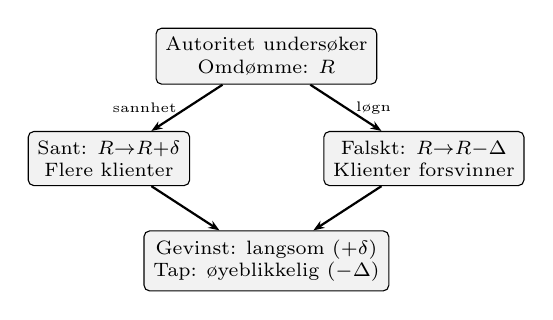
\begin{tikzpicture}[
    box/.style={draw, rounded corners=2pt, minimum width=2cm, minimum height=0.6cm, align=center, font=\scriptsize, fill=black!5},
    arr/.style={-{Stealth[length=4pt]}, thick}
]
\node[box] (exam) at (0,0) {Autoritet undersøker\\Omdømme: $R$};
\node[box] (true) at (-2,-1.3) {Sant: $R{\to}R{+}\delta$\\Flere klienter};
\node[box] (false) at (2,-1.3) {Falskt: $R{\to}R{-}\Delta$\\Klienter forsvinner};
\node[box] (insight) at (0,-2.6) {Gevinst: langsom ($+\delta$)\\Tap: øyeblikkelig ($-\Delta$)};

\draw[arr] (exam) -- node[left,font=\tiny] {sannhet} (true);
\draw[arr] (exam) -- node[right,font=\tiny] {løgn} (false);
\draw[arr] (true) -- (insight);
\draw[arr] (false) -- (insight);
\end{tikzpicture}
\caption{Anerkjent autoritet---asymmetriske insentiver.}
\label{fig:authority}
\end{figure}

\subsection{Flerdimensjonalt omdømme}

Omdømme er ikke en skalar, men en vektor på tvers av flere dimensjoner: økonomisk pålitelighet, personlig integritet, faglig kompetanse, samfunnsengasjement og andre (Fig.~\ref{fig:reputation-radar}). Ulike evalueringsleverandører projiserer denne vektoren ulikt avhengig av kontekst---en långiver prioriterer økonomisk pålitelighet, en arbeidsgiver faglig kompetanse, en nabo samfunnsatferd. Det finnes ingen enkelt ``korrekt'' omdømmeskår; bare perspektiver.

\begin{figure}[ht]
\centering
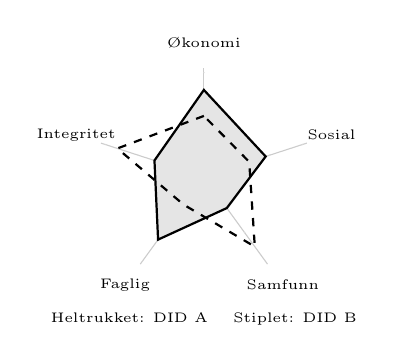
\begin{tikzpicture}[scale=0.55]
\foreach \a/\l in {90/Økonomi,162/Integritet,234/Faglig,306/Samfunn,18/Sosial} {
  \draw[gray!40] (0,0) -- (\a:2.5);
  \node[font=\tiny, align=center] at (\a:3.1) {\l};
  \foreach \r in {0.8,1.6,2.4} {
    \fill[black!15] (\a:\r) circle (0.5pt);
  }
}
\draw[thick, fill=black!10] (90:2.0) -- (162:1.2) -- (234:1.8) -- (306:0.9) -- (18:1.5) -- cycle;
\draw[thick, dashed] (90:1.4) -- (162:2.1) -- (234:0.8) -- (306:2.0) -- (18:1.1) -- cycle;
\node[font=\tiny] at (0,-3.3) {Heltrukket: DID A \quad Stiplet: DID B};
\end{tikzpicture}
\caption{Flerdimensjonale omdømmevektorer. Ulike DID-er utviser ulike profiler på tvers av dimensjoner.}
\label{fig:reputation-radar}
\end{figure}

\subsection{Demokratisert risikovurdering}

RSN demokratiserer systematisk risikovurdering---en kapabilitet som for øyeblikket er konsentrert i finansinstitusjoner, men anvendbar langt utover bankvirksomhet. Industrikonglomerater som vurderer leverandørpålitelighet, forsikringsselskaper som priser atferdsrisiko, aktsomhetsvurdering ved fusjoner og oppkjøp, estimering av utstyrs levetid i produksjon---hvor som helst motpartsrisiko krever vurdering, tilbyr RSN et desentralisert, markedsdrevet alternativ. Et marked av tolkningstjenester oversetter rå flerdimensjonale omdømmedata til handlingsrettede sammendrag, og gjør motpartsevaluering tilgjengelig for enhver deltaker til marginalkostnad.

% ============================================================
% 7. CONSENSUS AND DISPUTE RESOLUTION
% ============================================================
\section{Konsensus og tvisteløsning}

\subsection{Modell for desentralisert rettferdighet}

RSN omformulerer rettferdighet som et bilateralt forhandlingsproblem. Trusselen om permanent, verifiserbar omdømmeskade er et mer effektivt avskrekkingsmiddel enn rettssaker den skadelidte parten ikke har råd til.

\subsection{Emergent konsensus}

Hver deltaker opprettholder en personlig tilfredshetsterskel. Nettverkets samlede konsensus oppstår som det statistiske gjennomsnittet av tusenvis av bilaterale forhandlinger (Fig.~\ref{fig:consensus}). En respons langt over konsensus (barbarisk) er kostbar å publisere. En respons nær konsensus (proporsjonal) er billig. Konsensus er ikke en regel---det er et prissignal.

\begin{figure}[ht]
\centering
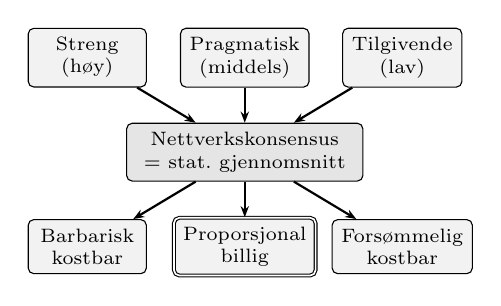
\begin{tikzpicture}[
    person/.style={draw, rounded corners=2pt, minimum width=1.5cm, minimum height=0.5cm, align=center, font=\scriptsize, fill=black!5},
    arr/.style={-{Stealth[length=4pt]}, thick}
]
\node[person] (a) at (-2,0) {Streng\\(høy)};
\node[person] (b) at (0,0) {Pragmatisk\\(middels)};
\node[person] (c) at (2,0) {Tilgivende\\(lav)};
\node[person, fill=black!10, minimum width=3cm] (cons) at (0,-1.2) {Nettverkskonsensus\\= stat.\ gjennomsnitt};
\node[person] (exp) at (-2,-2.4) {Barbarisk\\kostbar};
\node[person, double] (prop) at (0,-2.4) {Proporsjonal\\billig};
\node[person] (neg) at (2,-2.4) {Forsømmelig\\kostbar};

\draw[arr] (a) -- (cons);
\draw[arr] (b) -- (cons);
\draw[arr] (c) -- (cons);
\draw[arr] (cons) -- (exp);
\draw[arr] (cons) -- (prop);
\draw[arr] (cons) -- (neg);
\end{tikzpicture}
\caption{Emergent konsensus fra individuelle tilfredshetsterskler.}
\label{fig:consensus}
\end{figure}

\subsection{Kalibrering av straff}

Hver DID-innehaver erklærer offentlig responser på spesifikke kategorier av uredelighet. Uforholdsmessig harde eller milde erklæringer tiltrekker seg negative omdømmesignaler. Proporsjonale erklæringer godtas uten friksjon---et selvkalibrerende straffesystem.

Konsensuserklæringer er selv underlagt hykleri-deteksjon: å deklarativt forplikte seg til en konsensusposisjon mens man oppfører seg inkonsekvent, utgjør en omdømmeforseelse mer alvorlig enn det underliggende avviket, ettersom det demonstrerer forsettlig bedrag.

\subsection{Delegering}

Alle aktiviteter innenfor en DID---med ett unntak---kan delegeres til en annen DID. \textbf{Subjekt-rollen---DID-en hvis atferd påstanden handler om---kan ikke delegeres; den er uoverførbart bundet til identitetsinnehaveren som påstanden refererer til.} De andre aktive rollene---Utsteder, Autoritet, Vitne, Verifikator---kan overføres til en utpekt delegat-DID, enten for verifisering, innsending av påstander, konsensusdeltakelse eller tvisteløsning. Delegering er tilbakekallelig når som helst. Dette muliggjør spesialisering (f.eks. profesjonelle verifikasjonstjenester) mens Innehaveren beholder den endelige kontrollen og ansvaret. Delegering gjelder på tvers av hele systemet og er avgjørende for skalerbarhet.

\subsection{Fra individuell moral til emergent samfunnskontrakt}

Hver DID-s erklærte policy representerer en formalisering av individuell moral: hva Innehaveren anser som akseptabelt, hvordan de responderer på spesifikke atferder, hva de krever av motparter. Disse policyene pålegges ikke av en systemdesigner---de velges av hver deltaker og uttrykkes i maskinlesbar form.

Denne formaliseringen muliggjør en trinnvis fremvekst. For det første kodes individuell moral som \textbf{policy}---et sett med erklærte regler, terskler og responsfunksjoner som DID-en forplikter seg til å følge. For det andre produserer summen av alle policyer på tvers av nettverket \textbf{emergent etikk}---statistisk observerbare normer som ingen enkelt deltaker utformet, men som oppstår fra interaksjonen mellom tusenvis av individuelle moralske posisjoner~\cite{durkheim1893}. For det tredje utgjør denne emergente etikken, uttrykt som delte atferdsnormer håndhevet gjennom bilaterale prissignaler, en \textbf{målbar samfunnskontrakt}---ikke et teoretisk konstrukt som ingen signerte~\cite{rawls1971}, men et empirisk observerbart sett med regler støttet av faktisk atferd.

Denne prosessen speiler funn fra teorien om moralske grunnlag~\cite{haidt2012}: menneskelig moral er intuitiv, pluralistisk og kulturelt variabel. RSN krever ikke moralsk konsensus som en inngang; den produserer atferdskonsensus som en utgang. Den resulterende samfunnskontrakten er ikke statisk---den utvikler seg ettersom deltakere blir med, forlater og justerer sine policyer som respons på nettverkets tilbakemeldinger. I motsetning til klassisk samfunnskontraktsteori er denne kontrakten tilbakekallelig, observerbar og håndhevbar uten en suveren.

% ============================================================
% 8. ECONOMIC MODEL
% ============================================================
\section{Økonomisk modell}

De foregående avsnittene beskrev et verktøy---RSN-ets verifikasjonsmekanismer, kostnadsstruktur og emergente konsensus. Dette avsnittet beskriver en metodikk for å anvende dette verktøyet på finanspolitisk og styringsmessig overgang. Verktøyet er allsidig; metodikken nedenfor er én mulig anvendelse.

\subsection{Insentivstruktur}

Omdømme som kapital skaper direkte insentiver for ærlig atferd. I normal drift bygger deltakere omdømme naturlig gjennom dagligdagse transaksjoner og oppfylte forpliktelser. Den primære utgiften er på \emph{negative} påstander---registrering av skade forvoldt av andre. Denne asymmetrien insentiverer nyttig, pålitelig atferd: å være ærlig koster ingenting ekstra, mens å være skadelig skaper et dokumentert spor som andre vil betale for å bevare. Hykleri---å erklære regler uten å følge dem---er den mest kostbare feilmodusen, ettersom det demonstrerer forsettlig bedrag.

\subsection{Parallelt finanspolitisk system}

Tre komponenter muliggjør konkurransepress: (1)~\textbf{Enkel skatt}---en enkelt proporsjonal sats uten unntak, innledningsvis marginalt under den eksisterende effektive satsen; (2)~\textbf{Elektronisk registrering av offentlige utgifter (ESR)}---en inversjon av den tsjekkiske EET-modellen slik at borgere overvåker statens utgifter; (3)~\textbf{Borgerstyrt skattefordeling}---som starter på noen få prosent det første året og etter et tiår når alt fra lave tosifrede prosenter til en fullstendig migrering til et borgerstyrt system, avhengig av adopsjonstakten. Det faktiske tempoet avhenger av hastigheten hvormed frie markedsalternativer til statens tjenester oppstår, og av statens vilje til å samarbeide med overgangen; funksjonen av tid behøver ikke være lineær, og det er ingen grunn til å sette en øvre grense for hvor adopsjonen til slutt kan ende opp.

% ============================================================
% 9. MIGRATION PATH
% ============================================================
\section{Migreringsvei}

Migreringen forløper gjennom tre faser (Fig.~\ref{fig:migration}): \textbf{Fase~1: Overlegg} (RSN som informasjonslag, staten er eneste tilbyder), \textbf{Fase~2: Konkurranse} (RSN tilbyr funksjonelle alternativer, bruk av dobbelt system), og \textbf{Fase~3: Overgang} (RSN overgår statlige ekvivalenter, frivillig migrering). Overgangen er reverserbar på hvert trinn.

\begin{figure}[ht]
\centering
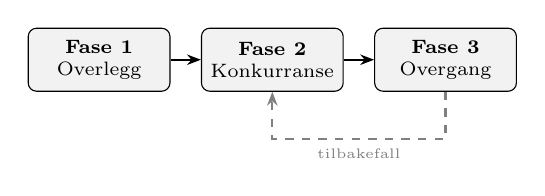
\begin{tikzpicture}[
    phase/.style={draw, rounded corners=3pt, minimum width=1.8cm, minimum height=0.8cm, align=center, font=\scriptsize, fill=black!5},
    arr/.style={-{Stealth[length=5pt]}, thick}
]
\node[phase] (p1) at (0,0) {\textbf{Fase 1}\\Overlegg};
\node[phase] (p2) at (2.2,0) {\textbf{Fase 2}\\Konkurranse};
\node[phase] (p3) at (4.4,0) {\textbf{Fase 3}\\Overgang};

\draw[arr] (p1) -- (p2);
\draw[arr] (p2) -- (p3);
\draw[arr, dashed, gray] (p3.south) -- ++(0,-0.6) -| node[below,font=\tiny,pos=0.25] {tilbakefall} (p2.south);
\end{tikzpicture}
\caption{Trefaset migrering---reverserbar på hvert trinn.}
\label{fig:migration}
\end{figure}

Den primære pressmekanismen er finanspolitisk: når betingede skattebetalere når en ``økonomisk signifikant minoritet $X$''---en gruppe stor nok til at undertrykkelse mot den forårsaker ikke-triviell økonomisk skade og sivil ulydighet blir en troverdig trussel---går staten inn i forhandling. Til illustrasjon bruker vi $X \approx 15\%$ av BNP, men den faktiske terskelen avhenger av den spesifikke økonomien.

% ============================================================
% 10. SECURITY ANALYSIS
% ============================================================
\section{Sikkerhetsanalyse}

Vi vurderer fem kategorier av motstandere: individuelle aktører med onde hensikter, organiserte grupper, bedriftsmotstandere, statsnivå-motstandere og protokollnivå-motstandere.

\textbf{Sybil-motstand}~\cite{douceur2002}. Å bygge omdømme krever vedvarende, verifiserbar interaksjon. Kostnaden ved et vellykket Sybil-angrep skalerer lineært med falske identiteter og kvadratisk med målets omdømmenivå. Å drive flere DID-er parallelt er mulig, men kostbart ved design---hver identitet må uavhengig akkumulere omdømme gjennom genuin aktivitet. I frie samfunn avskrekker denne kostnaden tilfeldig misbruk; i diktaturer blir parallelle DID-er et overlevelsesverktøy som muliggjør kompartmentalisert motstand, underjordisk koordinering og tryggere navigering på svartebørsen.

\textbf{Forsvar mot samarbeid.} Mønstre av gjensidig bekreftelse blant lukkede grupper er oppdagbare gjennom analyse av den sosiale grafen. Aggregeringsfunksjoner for omdømme nedvekter påstander fra tett klyngede kilder.

\textbf{Statsnivå-motstander.} Onion-ruting, fravær av sentralisert infrastruktur og fordeling av Verifikator-rollen på tvers av deltakerbasen sikrer at undertrykkelse krever tiltak uproporsjonale med enhver fordel.

\textbf{Personvern kontra ansvarliggjøring.} Pseudonymitet---en mellomting mellom anonymitet og identitetsavsløring---lar DID-er akkumulere meningsfullt omdømme uten å avsløre Innehaverens virkelige identitet.

% ============================================================
% 11. PRIVACY
% ============================================================
\section{Personvernhensyn}

RSN-ets personvernmodell er bygget på pseudonymitet. Innehaveren kontrollerer identitetsavsløring: minimal (rent pseudonym), selektiv (spesifikke legitimasjoner koblet) eller full (juridisk identitet assosiert). Publiserte påstander er permanente---systemet støtter kontekstuell korrigering, men ikke sletting. En Innehaver kan forlate en kompromittert DID og begynne på nytt, og gir dermed avkall på akkumulert omdømme.

% ============================================================
% 12. RELATED WORK
% ============================================================
\section{Relatert arbeid}

W3C DID Core-spesifikasjonen~\cite{did2022} og Ceramic Network~\cite{ceramic2023} gir identitetsgrunnlaget. EigenTrust~\cite{kamvar2003} demonstrerte distribuert omdømmeaggregering uten sentral autoritet. SBT-er~\cite{weyl2022} introduserte ikke-overførbare sosiale token. RSN skiller seg i sin vektlegging av økonomisk kostnad som et kvalitetsfilter og sin mekanisme for prising av radikalisme.

DAO-er~\cite{buterin2014} og kvadratisk stemmegivning~\cite{buterin2019} demonstrerte gjennomførbarheten av desentralisert styring. RSN utleder konsensus fra bilaterale prisforhandlinger snarere enn fra stemmegivning.

Forslaget bygger på anarkokapitalistisk teori~\cite{rothbard1973,hoppe2001} for privat tjenesteyting, men avviker på to kritiske punkter: det utformes for ondskap og gjengjeldende impulser snarere enn å anta rasjonalitet, og det foreslår gradvis overgang snarere enn revolusjon. Konseptet om emergente samfunnskontrakter har forløpere i Hayeks teori om spontan orden~\cite{hayek1973}.

\textbf{Anarko-agorisme.} RSN deler betydelig felles grunn med agoristisk motøkonomi~\cite{konkin2006}---særlig vektleggingen av å bygge parallelle institusjoner og frivillig utveksling. Agorisme har imidlertid en tendens til å anta rasjonell egeninteresse som en tilstrekkelig koordineringsmekanisme og mangler ofte en konkret migreringsvei fra eksisterende statsstrukturer. RSN innlemmer eksplisitt ikke-rasjonelle atferdstilbøyeligheter og gir en finanspolitisk pressmekanisme for gradvis overgang.

\textbf{Meritokrati.} RSN kan representere en første funksjonell beskrivelse av hvordan meritokrati~\cite{young1958} kan oppstå som en systemisk egenskap snarere enn et slagord. Tradisjonelle meritokratiske systemer svikter fordi de krever en sentral autoritet for å definere og håndheve ``fortjeneste''. I RSN oppstår fortjeneste fra bilaterale evalueringer: de som leverer verdi, akkumulerer omdømme; ingen komité bestemmer hvem som har fortjeneste.

\textbf{Eiendom som privilegium.} RSN avviker fundamentalt fra anarkokapitalistiske og østerrikske skolens behandlinger av eiendomsrett som naturlig og absolutt. I RSN-rammeverket er eiendom et \emph{privilegium}---en sosial anerkjennelse som i ekstreme tilfeller kan trekkes tilbake av fellesskapet når en deltaker fundamentalt bryter delte normer (svik, nektelse av å forsvare fellesskapet i en eksistensiell krise, systematisk utnyttelse). Dette er ikke statlig ekspropriasjon, men en tilbaketrekking av sosial anerkjennelse fra nettverket av bilaterale relasjoner.

% ============================================================
% 13. LIMITATIONS
% ============================================================
\section{Diskusjon og begrensninger}

\textbf{Kald start.} RSN-ets verdi avhenger av nettverkseffekter; tidlige brukere står overfor begrenset verdi inntil deltakelsen når en terskel. Selv fra tidlige stadier tjener imidlertid DID-nettverket som en nyttig supplerende informasjonskilde. Tidlig omdømmeevaluering og autoritetsvurdering forventes å utvikle seg gradvis med økende sofistikering.

\textbf{Anti-snylting og tilgangskontroll.} Mål-DID-er kan pålegge graderte gebyrer og tilgangsbegrensninger på spørringer fra DID-er med lavt omdømme. Dette er ikke binært, men en kontinuerlig skala: jo mindre omdømme en spørrende DID har, desto mindre informasjon mottar den, desto lenger venter den, og desto mer betaler den. Denne mekanismen insentiverer genuin deltakelse fremfor passiv konsumering.

\textbf{Ulikhet i tilgang.} Kostnaden ved å publisere påstander kan filtrere bort legitime klager fra økonomisk vanskeligstilte deltakere. Avhjelping: hver deltaker fungerer samtidig som en potensiell verifikator (eller delegerer denne rollen) og tjener verifikasjonsgebyrer. Over en tilstrekkelig tidshorisont bør en ikke-radikal deltaker nærme seg finansiell nøytralitet---verifikasjonsinntekter oppveier omtrent publiseringskostnader. Dette er en statistisk forventning, ikke en garanti.

\textbf{Ulikhet i omdømme.} Tidlige brukere akkumulerer fordeler som kan skape barrierer for de som kommer senere. Omdømmeevaluering utføres imidlertid av tredjepartsleverandører som kan velge å dempe førsteinngangsfordelen gjennom sine aggregeringsalgoritmer. Å være først med et godt omdømme er en legitim komparativ økonomisk fordel---og det er ved design.

\textbf{Åpne spørsmål.} Optimale kostnadsfunksjoner, aggregeringsstandarder, protokollstyring og interaksjon med AI-generert syntetisk omdømmedata forblir områder for fremtidig arbeid.

Denne artikkelen hevder ikke at RSN vil produsere optimale utfall under alle omstendigheter. Den hevder at RSN representerer et \emph{gjennomførbart} alternativ---teknisk implementerbart, økonomisk selvopprettholdende og sosialt kompatibelt med menneskelige atferdstilbøyeligheter slik de faktisk er.

% ============================================================
% 14. CONCLUSION
% ============================================================
\section{Konklusjon}

Denne artikkelen har presentert det omdømmebaserte sosiale nettverket, en desentralisert protokoll som muliggjør pseudonym, verifiserbar omdømmeutveksling. Prinsippet om kostbar radikalisme sikrer at svindelaktige påstander prises ut uten sensur. Den foreslåtte migreringsveien muliggjør gradvis, reverserbar overgang fra eksisterende institusjoner. Designet innlemmer menneskets natur slik den er---inkludert smålighet, ondskap og ønsket om gjengjeldende tilfredsstillelse---snarere enn å kreve ideologisk transformasjon. Resultatet er ikke utopi, men et system der rettferdighet er tilgjengelig, omdømme fortjenes, og kostnaden ved uredelighet bæres av den parten som forårsaket den.

% ============================================================
% REFERENCES
% ============================================================
\bibliography{references}

\end{document}
